\documentclass[10pt,a4paper,twocolumn]{article}
\usepackage[backend=biber,natbib=true,style=numeric,maxnames=50,sorting=none]{biblatex}
\usepackage{amsmath}
\usepackage{float}
\usepackage{authblk}
\usepackage{fancyhdr}
\usepackage{graphicx}

%%%%% Customize the below fields %%%%%
\usepackage[pdfauthor={ITU Journal Editors},
			pdftitle={Template for submitting papers to the ITU Journal on Future and Evolving Technologies},
			pdfsubject={ DESCRIBE SUBJECT HERE },
			pdfkeywords={One, two, three, four, five (List approximately five keywords in alphabetical order, separated by commas.},
			pdfproducer={International Telecommunication Union},
			hidelinks]{hyperref}
			
%%%%% do not touch %%%%%
\pagestyle{fancy}
\fancyhf{}
\rhead{{\footnotesize ITU Journal on Future and Evolving Technologies, Volume 0 (2022), Issue 0}}
\lfoot{© 2021 International Telecommunication Union}
\rfoot{\thepage}
\fancypagestyle{firstpage}{%
	\renewcommand{\headrulewidth}{0pt}
	\rhead{}
	\lfoot{}
	\rfoot{}
	\cfoot{{\tiny © International Telecommunication Union, 2021 \\
			Some rights reserved. This work is available under the CC BY-NC-ND 3.0 IGO license: \href{https://creativecommons.org/licenses/by-nc-nd/3.0/igo/}{https://creativecommons.org/licenses/by-nc-nd/3.0/igo/}\\
			More information regarding the license and suggested citation, additional permissions and disclaimers is available at:
			\href{https://www.itu.int/en/journal/j-fet/}{https://www.itu.int/en/journal/j-fet/}}}
}

% Keywords command
\providecommand{\keywords}[1]
{	
	\textbf{\textit{Keywords---}} #1
}

\date{}

%%%%% begin editing here %%%%%

% article specific packages
\usepackage{subcaption}
\usepackage{wrapfig}
\usepackage{tikz}
\usetikzlibrary{arrows}
\usetikzlibrary{snakes}
\usetikzlibrary{calc,patterns}

% article bibliography file
\addbibresource{bibliography-file.bib}

% title
\title{Template for submitting papers to the \\
	   ITU Journal on Future and Evolving Technologies}

% authors
\author[1,*]{ITU Journal Editors}
\author[1]{Secretariat}

% affiliations and corresponding author
\affil[1]{International Telecommunication Union}
\affil[*]{\small Corresponding author: journal@itu.int}

\def\abstract{\itshape}

\begin{document}
\thispagestyle{firstpage}
\twocolumn[
\begin{@twocolumnfalse}
	\maketitle
	\hrulefill \\
	\textit{\textbf{Abstract}---} 
	\begin{abstract}
		This template provides detailed instructions for submitting papers to the ITU Journal on Future and Evolving Technologies. Papers must be in American English and in black font. The abstract should appear in italics at the top, below the title and author's area. The abstract should normally contain 100 to 150 words, and in no case shall it exceed 200 words. All abbreviations and acronyms used in the abstract should be defined, and in the text the first time used. Do not cite references in the abstract.
	\end{abstract}
	\bigskip
	\keywords{One, two, three, four, five (List approximately five keywords in alphabetical order, separated by commas.}
	\bigskip
	\end{@twocolumnfalse}
]


\section{Introduction} 
\label{sec:intro}
\thispagestyle{firstpage}
This template provides detailed instructions for submitting papers to the ITU Journal: \textit{ICT Discoveries}. The next sections describe style, fonts and spacing to adopt. Please use this \LaTeX\ template for your paper. Additional instructions on submitting your paper can be found in the \href{https://www.itu.int/en/journal/Pages/submission-guidelines.aspx}{Author's Guidelines}. Please address any enquiries or suggestions about this template to the ITU Editorial Team at \href{mailto:journal@itu.int}{journal@itu.int}.


\section{Formatting}
\label{sec:sec2}
Papers must be within three to eight pages, including abstract, figures, tables and references.
Each paper must contain an abstract, which should approximately be between 100-150 words, and in no case, should it exceed 200 words.
All text, illustrations and charts must be kept within a print area of 17.5 cm/6.9 inches wide by 24.4 cm/9.6 inches high.
Do not write anything outside the print area.
The top margin must be 2.5 cm, and the left and right margins must be 1.5 cm.
All text must be in a two-column format.
Columns are to be 8.5 cm wide, with a 1 cm space between them.
Text must be fully justified, A4 size (21 cm wide by 29.7 cm long, or 8.27 inches by 11.7 inches).
If the last page of your paper is only partially filled, arrange the columns so that they are evenly balanced if possible, rather than having one long column.
The balancing can be achieved using the \texttt{\textbackslash balance} command before the last section of the left column of the last page.\footnote{This command should be avoided if footnotes appear at the bottom of the left column of the last page.}


\section{Title page section}
\label{sec:sec3}
The paper title should be \texttt{Large} size, uppercase, and bold face, as shown in this template.\footnote{NEEDS TO BE UPDATED}
The authors' name(s) and affiliation(s) are to appear below the title in capital and lower case letters, in \texttt{large} size, keeping the spacing as indicated in the template instructions.



\section{Type-style and fonts}
\label{sec:sec4}
Text should appear in Cambria font\footnote{NEEDS TO BE UPDATED}, size 10-point, with single spacing, apart from headings.
This is already implemented as default in the template.
To be able to obtain the Cambria character \textbf{compile using XeLaTeX}, instead of pdflatex.\footnote{CAN BE REMOVED}
To obtain the proper paragraph spacing, please insert an empty line in the \LaTeX~ source file.


\section{Major headings}
\label{sec:sec5}
Major headings (for example, ``1. INTRODUCTION'') are predefined in the template, and \textbf{should not} be changed.

%%= subsection example =%%
\subsection{Subheadings}
\label{ssec:sec5.1}
Subheadings are predefined in the template, and \textbf{should not} be changed.

%%= subsubsection example =%%
\subsubsection{Sub-subheading}
\label{sssec:sec5.1.1}
Sub-subheadings, as in this paragraph, are discouraged.
However, if you must use them, they should appear as predefined in the template, and \textbf{should not} be changed.


\section{Images}
\label{sec:sec6}
Images (figures and tables) can be either in color or black and white.
Images must appear within the designated margins.
Caption and number every image.
Figure captions must be placed on the bottom, not top, of the figure.
Table captions must be located on the top of the table.
Keep titles with images. 

%%= example figure =%%
\begin{figure}
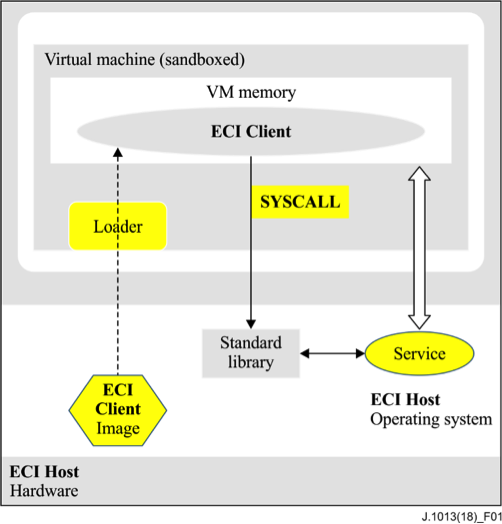
\includegraphics[width=\columnwidth]{Figure1}
\caption{ECI Host - Hardware}\label{fig:fig1} 
\end{figure}
%%======%%


And for a table:
%%= example table =%%
\begin{table}
\caption{Table title style}\label{tab:tab1} 
\begin{small}
	\begin{tabular}{|c|c|}
		\hline
		Character & Entity Reference\\ 
		& \\
		\hline
		\hline
		\& & \&amp; \\
		\hline
		< & \&lt;\\
		\hline
		> & \&gt; \\
		\hline
		``  & \&quot; \\
		\hline
		` & \&apos; \\
		\hline
	\end{tabular}
\end{small}
\end{table}
%%======%%


And an equation:
%%= example equation =%%
\begin{equation}\label{eq:eq1}
	PL(D)=PL(D)+10\log 
\end{equation}
%%======%%


\section{Footnotes}
\label{sec:sec7}
Use footnotes sparingly (or not at all!)\footnote{To obtain the right formatting for the footnotes, use the predefined command \texttt{\textbackslash{footnote}}}.
To help your readers, avoid using footnotes altogether and include necessary peripheral observations in the text (within parentheses, if you prefer, as in this sentence).


\section{Using references}
\label{sec:sec8}
List and number all bibliographical references at the end of the paper, and refer to them in the text as shown in this sentence \cite{wiegand2019WHO}.


\section{Page numbering}
\label{sec:sec9}
Please number all pages of your paper.


\section{Authoring recommendations}
\label{sec:sec10}
Define abbreviations and acronyms the first time they are used in the text, even if they have already been defined in the abstract.
Abbreviations and acronyms should be avoided in the title.

Units should be expressed as much as possible in international units, and a dot (``.'') should be used to express decimal points (not ``,'').


\section{Conclusion}
\label{sec:sec11}
The main conclusions may be presented in a short final section.


\section*{Acknowledgements}
\label{sec:ackn}
You may list here colleagues, sponsors and financial supporter that you wish to acknowledge.
This section is not required.


\printbibliography


\section*{Authors}
\label{sec:auth}


\end{document}
